\documentclass[a4paper]{article}
\usepackage[T1]{fontenc}
\usepackage{amsmath}
\usepackage{hyperref}
\usepackage{amsthm}
\usepackage{amssymb}
\usepackage{float}
\usepackage[utf8]{inputenc}
\usepackage[italian]{babel}
\usepackage{graphicx} 
\graphicspath{{figures/}}
\newcommand{\lcc}{\textit{largest connected component}}
\begin{document}

\author{
	Lorenzo Dentis, \textit{lorenzo.dentis@edu.unito.it}\\
	Roberto Casale, \textit{roberto.casale719@edu.unito.it}\\
	Alessandro Nocera, \textit{alessandro.nocera@edu.unito.it}
}
\title{Relazione progetto Network Science}
\maketitle

\tableofcontents

\section{appunti da scrivere ordinatamente nelle sezioni}
Degree correlation: tendenza a nodi con un certo degree a connettersi a nodi con un degree simili o uguale
ci aspettiamo che sia assortativa perchè abbiamo una grossa gigant component e una core perifery structure


Comunities:set di nodi molto interconnessi
ci aspettiamo tante comunità
abbiamo 218 comunità (tante) quindi non abbiamo dei super hub, ne abbiamo solo 2

\section{Analisi}
\subsection{Dataset}
Il dataset che abbiamo analizzato è il seguente: \href{http://snap.stanford.edu/data/loc-brightkite.html}{ Friendship and Mobility: User Movement in Location-Based Social Networks }(E. Cho, S. A. Myers, J. Leskovec.).\\
Contiene dati anonimi estratti dal social-network \textit{Brighthike}, un social basato sulla posizione.
In qualsiasi momento un utente ha la possibilità di condividere la sua posizione e cercare altre persone geograficamente vicine che fanno uso di quel social, c'è anche la possibilità di segnalare che si è stati in un posto preciso ad una data ora.
Il dataset preso in esame è una restrizione di questi dati secondo 3 filtri:
\begin{itemize}
	\item Temporale: Sono presenti solo risultati raccolti tra Apr. 2008 e Ott. 2010.
	\item Spaziale: In generale tutte le coordinate si riferiscono a luoghi interni agli USA, ci sono però delle rare eccezioni, come mostrato in figura \ref{FIG:posizione_generica}
		\begin{figure}[!ht]
			\centering
			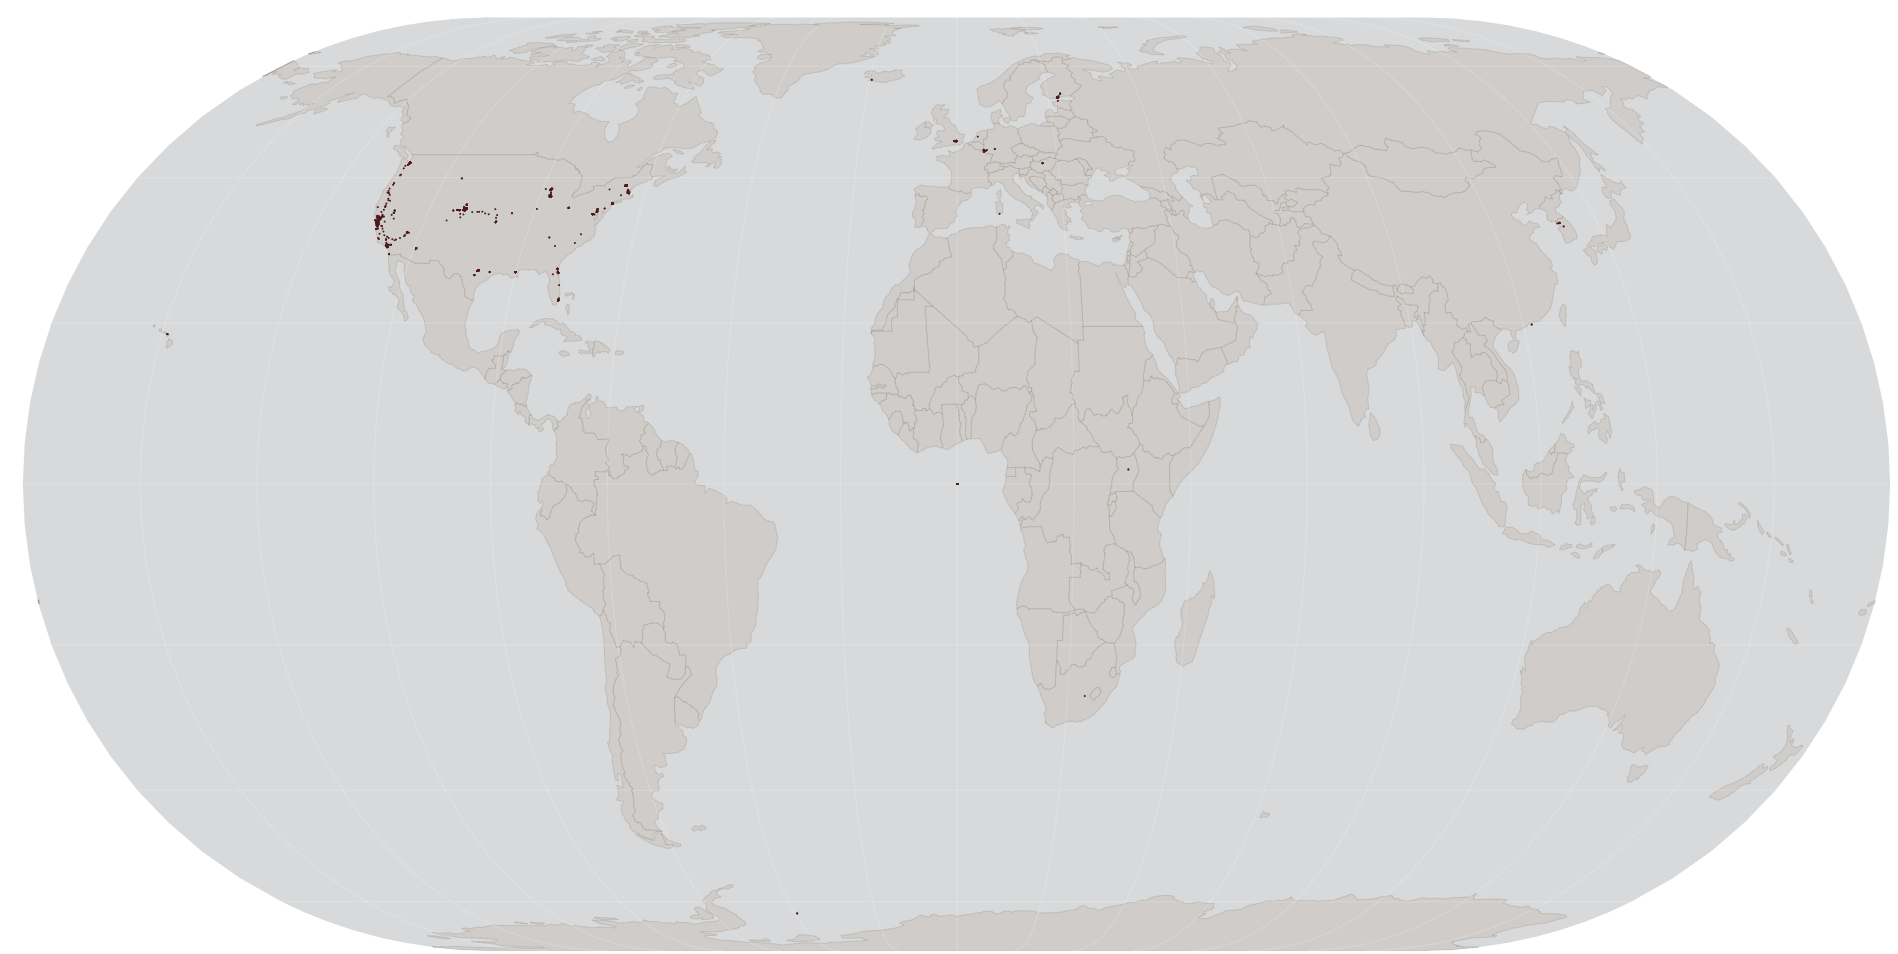
\includegraphics[width=\linewidth]{posizione_generica}
			\caption{mappa con coordinate}
			\label{FIG:posizione_generica}
		\end{figure}
		Non vi è una spiegazione ma si possono fare delle ipotesi, il social potrebbe essersi diffuso solo in America e negli Stati Europei molto meno.
		L'ipotesi che ci sentiamo di avanzare è che i dati raccolti siano solo di utenti Americani ed i luoghi \textit{outliers} siano luoghi in cui l'utente ha viaggiato (molti di questi sono luoghi turistici)
	\item Sociale: Sono stati mantenuti solo gli archi che indicavano incontri, quindi se un nodo ha effettuato \textit{check-in} in un dato luogo ma nessuno era presente il dato è stato eliminato.
		Questo fa si che sia possibile avere archi duplicati (due persone che si incontrano diverse volte in luoghi diversi o momenti diversi) ed archi monodirezionali, ad esempio un utente potrebbe aver guardato se ci fosse qualcuno nelle vicinanze e poi non averlo contattato.\\
		Tutti gli archi monodirezionali sono stati trasformati in bidirezionali perchè per lo scopo della ricerca era importante registrare gli incontri, che questi fossero o meno rappresentativi di una interazione sociale
\end{itemize}

\subsection{Dataset e approssimazioni}
Il dataset è composto da $58228$ nodi e $214078$ archi, rappresentanti un incontro tra due nodi, ciò lo rende a volte intrattabile ma fornisce anche la possibilità di effettuare operazioni di approssimazione e vedere come queste si comportano rispetto a differenti misure.
L'operazione di approssimazione più efficace che abbiamo trovato è stata la scelta di ridurre il dataset ai soli dati raccolti in un anno (2009), ciò ha portato ad un dimezzamento dei nodi (24568 nodi e 19898 archi) rendendo possibili computazioni troppo dispendiose altrimenti.
E' stato generato anche una terzo dataset, andando a focalizzarsi sui luoghi visitati, difatti tali luoghi possono essere visti come \textit{foci} ed hanno un grosso impatto sul meccanismo di creazione degli archi.

\subsection{Distanze}
Questa è stata la prima operazione che ha richiesto una approssimazione, difatti è stato usato il grafo relativo ai dati del solo anno $2019$, dovendo cercare uno shortest path per ogni coppia di nodi l'algoritmo di \textit{path finding} verrebbe eseguito potenzialmente $n*(n-1)$, cioè $3^.363^.942^.000$. ($n$ è il numero di nodi facende parte della \textit{largest connected component}, brevemente \textit{lcc}.
Il grafo non è completamente connesso, ma un rapido controllo ha indentificato che il 96\% dei nodi si trovavano nella \lcc, quindi analizzare il grafo completo è computazionalmente troppo intensivo.


Il calcolo delle distanze sul dataset ridotto ha fornito misure in linea con quanto ci si aspettava, il diametro (il più lungo shortest path) è $16$ mentre la media è molto bassa, $1,103$. Questo valore si spiega analizzando le componenti fortemente connesse.
Vi è infatti una enorme componente connessa massimale, ma quasi tutti i nodi rimanenti sono in \textit{clusters} molto piccoli, addirittura di sole due persone. Questo abbassa tantissimo la media perciò risulta molto più interessante studiare l'\textit{average\_shortest\_path} della sola componente massimale.\\
Questi risulta essere $5,71$ in linea con l'esperimento effettuato da Stanley Milgram che rilevava 6 gradi di separazione tra tutte le coppie di nodi, in questa rete la \textit{small world hypothesis} è confermata. 

\subsection{Componenti connesse}
Analizzando tutte le componenti formtemente connesse ne individuiamo $547$, di seguito una lista delle prime 10 in ordine decrescente di dimensione.\\
\begin{tabular}{ | c | c | c | c | c | c | c | c | c | c | }
  \hline
  56739 & 49 & 11 & 11 & 10 & 10 & 9 & 8 & 8 & 7\\
  \hline
\end{tabular}\\
Il 96\% dei nodi fa parte della \lcc, tutte le altre componenti connesse sono formati da meno di 3/4 nodi. 
Ci sono due differenti possibilità per spiegare questo fenomeno (le due possibilità saranno analizzate meglione nella sezione CITARE LA SEZIONE STUDIO DEI FOCI): Esiste un luogo geografico dove molte persone si sono incontrate (cioè molti utenti vivono in una area geografica ridotta) oppure esistono degli hub, degli utenti che si sposano molto ed incontrano molte persone.
%TODO: ipotesi:potrebbero essere tutti vicini geograficamente oppure la "classe" dei nodi, oppure per via degli hub presenti oppure ci sono luoghi molto trafficati, plottare 

\subsection{analisi dei Degrees}
Avendo una componente connessa molto grande ed essendo questa una rete sociale ci aspettavamno una struttura \textit{core-perifery} quindi alcuni \textit{super-hubs} aventi un grado molto elevato ed una maggioranza dei nodi con un degree molto basso.
Questo è confermato dalla media dei gradi di tutti i nodi del grafo: $7.35$.
Un valore inaspettatamente basso ma che si spiega andando a verificare quanti nodi hanno pochi vicini, i nodi che hanno meno di 4 vicini sono $39586$ e quelli che ne hanno solo 1 sono $21157$, il $36\%$ dei nodi ha un solo collegamento.
Viene identificata quindi una fortissima struttura \textit{core-perifery} dove i nodi che non fanno parte del \textit{core} sono quasi completamente esclusi.
Andando ad effettuare il plot \ref{FIG:degree_dist_G} si evidenzia la distribuzione \textit{Heavy-tail} che ci aspettiamo dalle precedenti osservazioni, la maggior parte dei nodi ha un grado molto basso mentre sono molti pochi i nodi ad avere un grado maggiore di $10^2$.
\begin{figure*}[!ht]
\centering
\makebox[\textwidth][c]{
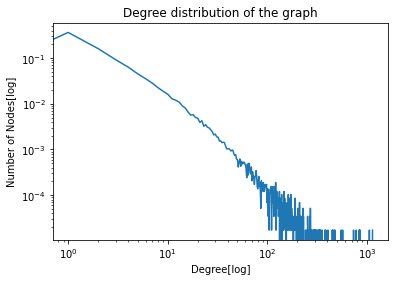
\includegraphics[width=0.85\textwidth]{degree_distribution.png}
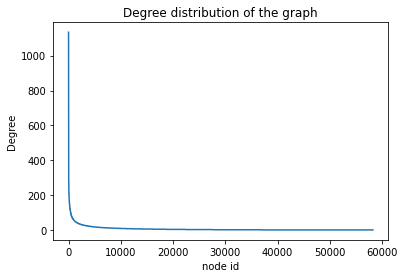
\includegraphics[width=0.85\textwidth]{nodes_degree.png}}
\caption{Degree distribution of graph} \label{FIG:degree_dist_G}
\end{figure*}
Ci sono alcui dettagli notevoli (che abbiamo notato solo dopo analisi di assortatività), in primis il numero hub è molto basso, ci sono 7 nodi che possiamo realmente definire hub (cioè nodi il cui grado è >> del grado di tutti gli altri), il secondo dettaglio è che i pochi hub hanno comunque pochi vicini.
Il massimo degree calcolato è $1134$ che è lo $0.5\%$ di tutti i link, ciò potrebbe essere dovuto al fatto che il grafo è poco connesso, ma gli studi effettuati sulla dimensione della \lcc lo escludono, la conclusione è che in questa rete non ci sono hub molto grandi.
%TODO: è una power-law?
\subsection{Clustering coefficient e Degree correlation}
Queste due differenti analisi sono inserite nella stessa sezione in quanto hanno fornito risultati inaspettati, che hanno richiesto un'analisi più approfondita prima di essere spiegabili.
Il clusering coefficient è risultato essere $0.172$, un valore molto basso che indicava una scarsa tendenza dei nodi a rispettare la \textit{triadic clousure}.
Essendo questa una rete sociale ci aspettavamo un valore molto alto, ad indicare che se un nodo $a$ è collegato al nodo $b$ ed un nodo $c$ è collegato al nodo $a$ è molto probabile che ci sia un collegamento tra $c$ e $b$.
Alla luce di ciò abbiamo calcolato quanti triangoli del tipo $a - b - c$ fossero presenti nel grafo e ne abbiamo individuati $494728$ di cui solo $19685$ chiusi, il $3.98\%$.
La prima ipotesi per giustificare questo numero è stata la possibilità che il grafo rappresentasse un sottografo di una rete sociale, in termini semplici non è detto che le persone che un individuo frequenta online siano poi le persone con cui si incontra, è possibile che gli utenti di \textit{Brighthike} comunicassero senza incontrarsi di frequente.
Ma questa ipotesi non è molto sensata e soprattutto non è supportata da nessun dato, anzi per il fenomeno dell'affiliazione persone con \textit{foci} in comune dovrebbero tendere a formare legami sociali (il social Brighthike è un esempio di \textit{focus}).


L'ipotesi corretta, derivata dallo studio dell'assortatività e confermata dalla lettura del paper orginale, è che gli incontri tra individui non siano una forte rappresentazione della rete sociale sottostante.\\
Anche l'assortatività riporta una misura inaspettata, avendo questa un valore pari a $0.0108$ identifica che la rete non è assortativa come ci saremmo aspettati da una rete sociale, bensì molto più simile ad un random network.
I nodi quindi non tendono a rispettare alcun criterio di assortatività, non c'è alcuna relazione tra la presenza di un arco e il grado dei nodi ai capi dello stesso.
La spiegazione di ciò la si può trovare leggendo il paper orginale: 
"We show that social relationships can explain about 10\% to 30\% of all human movement, while periodic behavior explains 50\% to 70\%"\\ %TODO: bibliografia e citare
Quindi questo dataset non rappresenta perfettamente una rete sociale, pur mantenendo molte delle caretteristiche che ne definiscono una.
Essendo gli incontri tra utenti tra il 50\% ed il 70\% dovuti alla "routine" (e quindi non rappresentanti una rete sociale sottostante) molti di questi mettono randomicamente in relazione nodi che in realtà non hanno alcun legame.

\subsection{Analisi delle comunità}
Posto che la rete somiglia più ad un network randomico che ad una rete sociale, come è possibile che molte caratteristiche ? (brevi distanze, componenti fortemente connesse, Heavy-tail distribution).\\
Per rispondere abbiamo analizzato le comunità, in particolare abbiamo considerato solo la \lcc, dato che già sappiamo che la maggior parte dei nodi non appartenenti alla \textit{lcc} compongono \textit{clique} da 2-4 nodi disconnesse dal resto del grafo.
É stato rilevato un numero di comunità variabile tra le $150 \text{ e le } 220$, la maggior parte di piccole dimensioni (più dei 3/4 avente una dimensione massima di 100 nodi), il valore non è fisso in quanto per il calcolo è stato usato l'algoritmo di $Louvain$ che ha una assegnazione iniziale randomica.
Come mostrato in figura \ref{FIG:communities_sizes} è presente una distribuzione \textit{Heavy-tail} delle dimensioni della comunità.
In sintesi abbiamo poche comunità di nodi, alcune di queste molto grandi.
All'interno di queste comunità ci sono molti collegamenti, un \textit{average shortest path} molto breve che permette di attraversarle molto in fretta, e le comunità sono collegate tra loro seguendo una struttura tendente ad essere \textit{Hubs-and-spoke}, cioè esistono delle grandi comunità a cui sono connessi molte altre comunità più piccole. \\
\begin{figure*}[!ht]
\centering
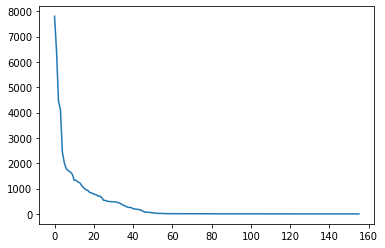
\includegraphics[width=0.7\textwidth]{community_size.png}
\caption{size of communities} \label{FIG:communities_size}
\end{figure*}\\
Tutte queste caratteristiche si osservano bene andando a costruire un grafo con le comunità come nodi.
Calcolando su questo grafo la degree correlation otteniamo un valore pari a $-0.533$ che tende ancora di più a $-1$ se consideriamo tutto il grafo e non solo la \lcc ed andando a effettuare un plot del nuovo grafo notiamo subito la struttura \textit{Hubs-and-spoke}
In figura \ref{FIG:communities_plot} sono rappresentate le comunità, le etichette degli archi identificano le comunità in ordine decrescente di dimensione (0 la più grande) e il layout è basanto sull'algoritmo \textit{spring} di Fruchterman-Reingold, cioè più un nodo è distante dall'altro minori archi ci sono che collegano le due comunità.

\begin{figure*}[!ht]
\centering
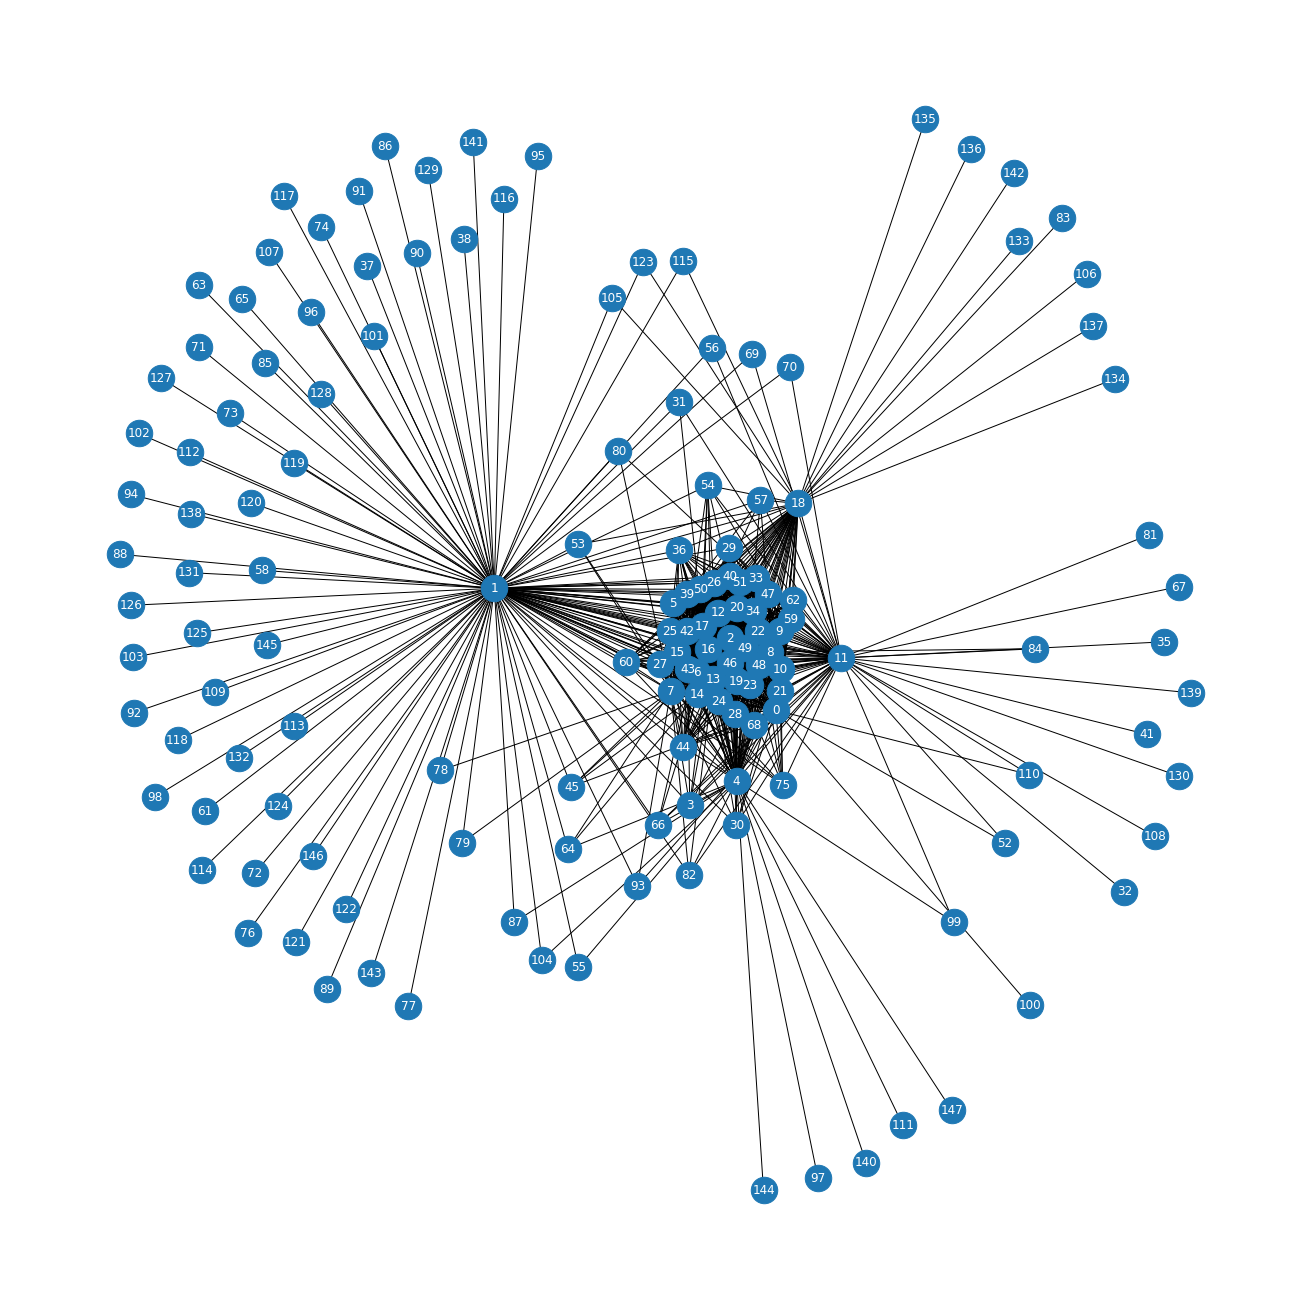
\includegraphics[width=1\textwidth]{cummunity_plot.png}
\caption{Plotting with communities as node} \label{FIG:communities_plot}
\end{figure*}


La prima cosa che si nota è che il \textit{Degree} di una comunità è proporzionale alla sua dimensione, %TODO:aggiungere altro.

\subsection{analisi di centralità}
%C'è poco da dire
\subsection{analisi di affiliazione}
L'ultima interessante analisi svolta è stata l'analisi di affiliazione, essendo un dataset relativo a luoghi frequentati da individui l' analisi più interessante è quella dei luoghi.
I luoghi possono infatti essere visti come dei \textit{foci} ed un'analisi dei luoghi più frequentati e dei nodi che frequentano tali luoghi può fornire risultati interessanti.
Il primo risultato interessante ottenuto è che ci sono dei luoghi dove moltissime persone si sono incontrate, il luogo più frequentato ha avuto $2606$ distinti visitatori, il $9\%$ di tutti i nodi. Il 30\% degli individui ha visitato almeno uno dei 4 luoghi più frequentati, si nota che zone corrispondono alle zone più popolose (il luogo dove si sono incontrate più persone ad esempio è il centro di Denver).
%TODO: che altre analisi si possono fare?
\section{Simulazione dinamica}
\end{document}

